\documentclass{ENSEIRB_poster}

\usepackage[utf8]{inputenc}

%% TODO: Mettre le titre de votre PFE
\title{Machine Learning Operations (MLOps) au sein de "HomeByMe"}
%% TODO: Mettre vos nom et prénom
\author{El Osrouti Fatima Ezahrae}

%% TODO: Mettre le chemin vers votre photo
\newcommand{\authorpicture}[0]{./logos/id.jpeg}

%% TODO: Mettre le nom de votre tuteur pédagogique
\newcommand{\tuteur}[0]{Janin David}

%% TODO: Mettre le nom de votre responsable de stage
\newcommand{\encadrant}[0]{Buffet Jean}

%% TODO: Mettre votre filière Electronique, Informatique, Mathématique, 
%% ou Télécom
\newcommand{\filiere}[0]{Informatique}

%% TODO: Mettre le nom de votre option de 3ème année
%% Pour les infos: PRCD, RSR, TMJV, GL, ... ou Etranger si vous avez
%% fait une année à l'étranger.
\newcommand{\option}[0]{Etranger}

%%
%% Ligne de logo(s) à la fin du poster pour mettre le logo de
%% l'entreprise dans laquelle s'est effectué le stage et ses
%% partenaires éventuels.
%%
% Définir la longueur suivant #logo (ici 4)
%%  \onecolwidth, \twocolwidth, \threecolwidth or \fourcolwidth (see ENSEIRB_poster.cls)
\setlength{\bottomcolwidth}{\fourcolwidth}

\setbeamertemplate{footline}{
  \begin{beamercolorbox}[wd=\paperwidth,colsep=0.2cm]{bottomrulerbox}\end{beamercolorbox}
  \vspace{0.5in}
  \begin{columns}[c]
    % First logo
    \begin{column}{\bottomcolwidth}
      \centering
      %%
\includegraphics[height=3cm]{logos/logo_BordeauxINP}
      
\includegraphics[height=3cm]{logos/logo_em}
    \end{column}
    % Second logo
    % \begin{column}{\bottomcolwidth}
    %   \centering
    %   
\includegraphics[height=3cm]{logos/logo_cnrs}
    % \end{column}
    % Third logo
    \begin{column}{\bottomcolwidth}
      \centering
      
\includegraphics[height=3cm]{templateLatex/logos/3DS_3DVIA_Logotype_RGB_Black.png}
    \end{column}
    % Fourth logo
    \begin{column}{\bottomcolwidth}
      \centering
      
\includegraphics[height=3cm]{templateLatex/logos/logoDassault.png}
    \end{column}
    %end
  \end{columns}
      {}
      \vspace{2cm}
}


\begin{document}

\begin{frame}[t] % The whole poster is enclosed in one beamer frame

  % The whole poster consists of sections of one, two or three columns. Choose the appropriate width :
  % \onecolwidth, \twocolwidth, \threecolwidth, or \fourcolwidth
  % correspond to the width of one column when there are 1, 2, 3 or 4 columns in parallel.
  % You can even use \twothirdcolwidth when you want to distribute 
  % two columns with 2/3 and 1/3
  %
  % spacing empty columns of size \sepwidth should be inserted on both sides and between columns if you want to have a clean positioning of the columns.

  \begin{columns}[c] 
    \begin{column}{\sepwidth}\end{column} % Empty spacer column

    \begin{column}{\threecolwidth}
      \begin{block}{Marques Dassault Systèmes}
        \begin{figure}
          \includegraphics[width=.35\linewidth]{templateLatex/logos/3DS_2021_3DEXP BRAND PLATFORM_WHITE_RGB_JAN.png}
          \caption{Jean de La Fontaine par Hyacinthe Rigaud, en 1690.}
        \end{figure}
      \end{block}
    \end{column}

    \begin{column}{\sepwidth}\end{column} % Empty spacer column

    \begin{column}{\twothirdcolwidth}
      \begin{alertblock}{L'auteur: EL Osrouti Fatima Ezahrae}
        Élève ingénieure en 3ème années à l'Enseirb-matmeca filière informatique. J'ai effectué ma 3ème année en échange à l'uinversité technique de Berlin où j'ai pris principalement des cours d'intelligence artificielle et de données.
        % \begin{flushright}
        %   \small{[source: Wikipedia]}
        % \end{flushright}
      \end{alertblock}
      
      \begin{block}{Stage}
        %Ce poster s'intéresse à la fable ``Le Faucon et le Chapon''. Il s'agit de la vingt-et-unième fable du livre VIII de Jean de La Fontaine situé dans le second recueil, édité pour la première fois en 1678. Le choix de cette fable est purement aléatoire. Elle serait imitée des contes indiens de Bidpaï et Lokman.
        Définir et mettre en oeuvre un service qui permettra l'automatisation complète d'un systèùe d'IA au sein De HomeByMe pour la collecte, le traitement des données, l'ingénieurie des fonctionnalités, l'étiquetage des données, la conception de modèles, formation et optimisation de modèles, déploiement et surveillance des terminaux
      \end{block}
    \end{column}

    \begin{column}{\sepwidth}\end{column} % Empty spacer column
  \end{columns}

  % ------------ Horizontal separation for changing number of columns in the width ------------

%%  \begin{columns}[c] 
%%    \begin{column}{\sepwidth}\end{column} % Empty spacer column
%%  \end{columns}

  % ------------ Changing number of columns in the width ------------

  \begin{columns}[t]
    \begin{column}{\sepwidth}\end{column} % Empty spacer column

    \begin{column}{\twocolwidth}
      \begin{block}{Dassault Systèmes}
        Fondée en1981, initialement une division de Dassault Aviation.\\
        Développement de logiciels de conception 3D \\
        Maquettes numériques et solutions de gestion du cycle de vie des produits (PLM).\\ 
        Possède 12 marques, dont 3DVIA, qui a comme produit HomeByMe.
        % Une traîtresse voix bien souvent vous appelle ;\newline
        % Ne vous pressez donc nullement :\newline
        % Ce n’était pas un sot, non, non, et croyez-m’en,\newline
        % Que le Chien de Jean de Nivelle.
      \end{block}

      \vspace{5pt}

      \begin{alertblock}{HomeByMe}
        % \textbf{Jean de Nivelle} (1422 -- 26 juin 1477) également connu sous le nom de Jean III (Ier) de Montmorency-Nevele, est un personnage français du Moyen Âge (XVe siècle) à l'origine de l'expression populaire \emph{être comme ce chien de Jean de Nivelle (qui fuit quand on l'appelle)} et dont le nom apparaît dans plusieurs chansons traditionnelles françaises.
        \textbf{HomeByMe} est une plateforme en ligne qui permet de créer des plans 2D ou 3D pour des projets d'aménagement intérieur. \\
        Les utilisateurs peuvent concevoir des espaces virtuels, meubler et décorer les pièces, et visualiser le résultat.\\
        Les clients cibles sont des particuliers, des architectes, des designers ou des entreprises tel que Conforama, Leroy Merlin...
      \end{alertblock}

      \vspace{5pt}

      %\begin{block}{Mise en place du décor}
      \begin{block}{Jumeau virtuel}
        La stratégie du jumeau virtuel chez Dassault Systèmes repose sur la création de répliques numériques de produits ou systèmes physiques. Ces jumeaux virtuels permettent de simuler, tester, et optimiser des conceptions avant même leur fabrication réelle. Cela accélère l'innovation, réduit les coûts, et améliore la durabilité en permettant des ajustements continus basés sur des données réelles, tout au long du cycle de vie des produits.\\
        Un des outils de réalisation du jumeau virtuel est l'intelligence artificielle(IA).
        % Un citoyen du Mans, chapon de son métier\newline
        % Était sommé de comparaître\newline
        % Par-devant les lares du maître,\newline
        % Au pied d’un tribunal que nous nommons foyer.\newline
        % Tous les gens lui criaient, pour déguiser la chose :\newline
        % \begin{quote}
        %   `` Petit, petit, petit ! ''
        % \end{quote}
        % Mais, loin de s’y fier,\newline
        % Le Normand et demi laissait les gens crier.\newline
        % \begin{quote}
        %   `` Serviteur, disait-il ; votre appât est grossier :
        %   On ne m’y tient pas ; et pour cause.''
        % \end{quote}
      \end{block}

    \end{column}

    \begin{column}{\sepwidth}\end{column}

    \begin{column}{\twocolwidth}
    \begin{figure}
        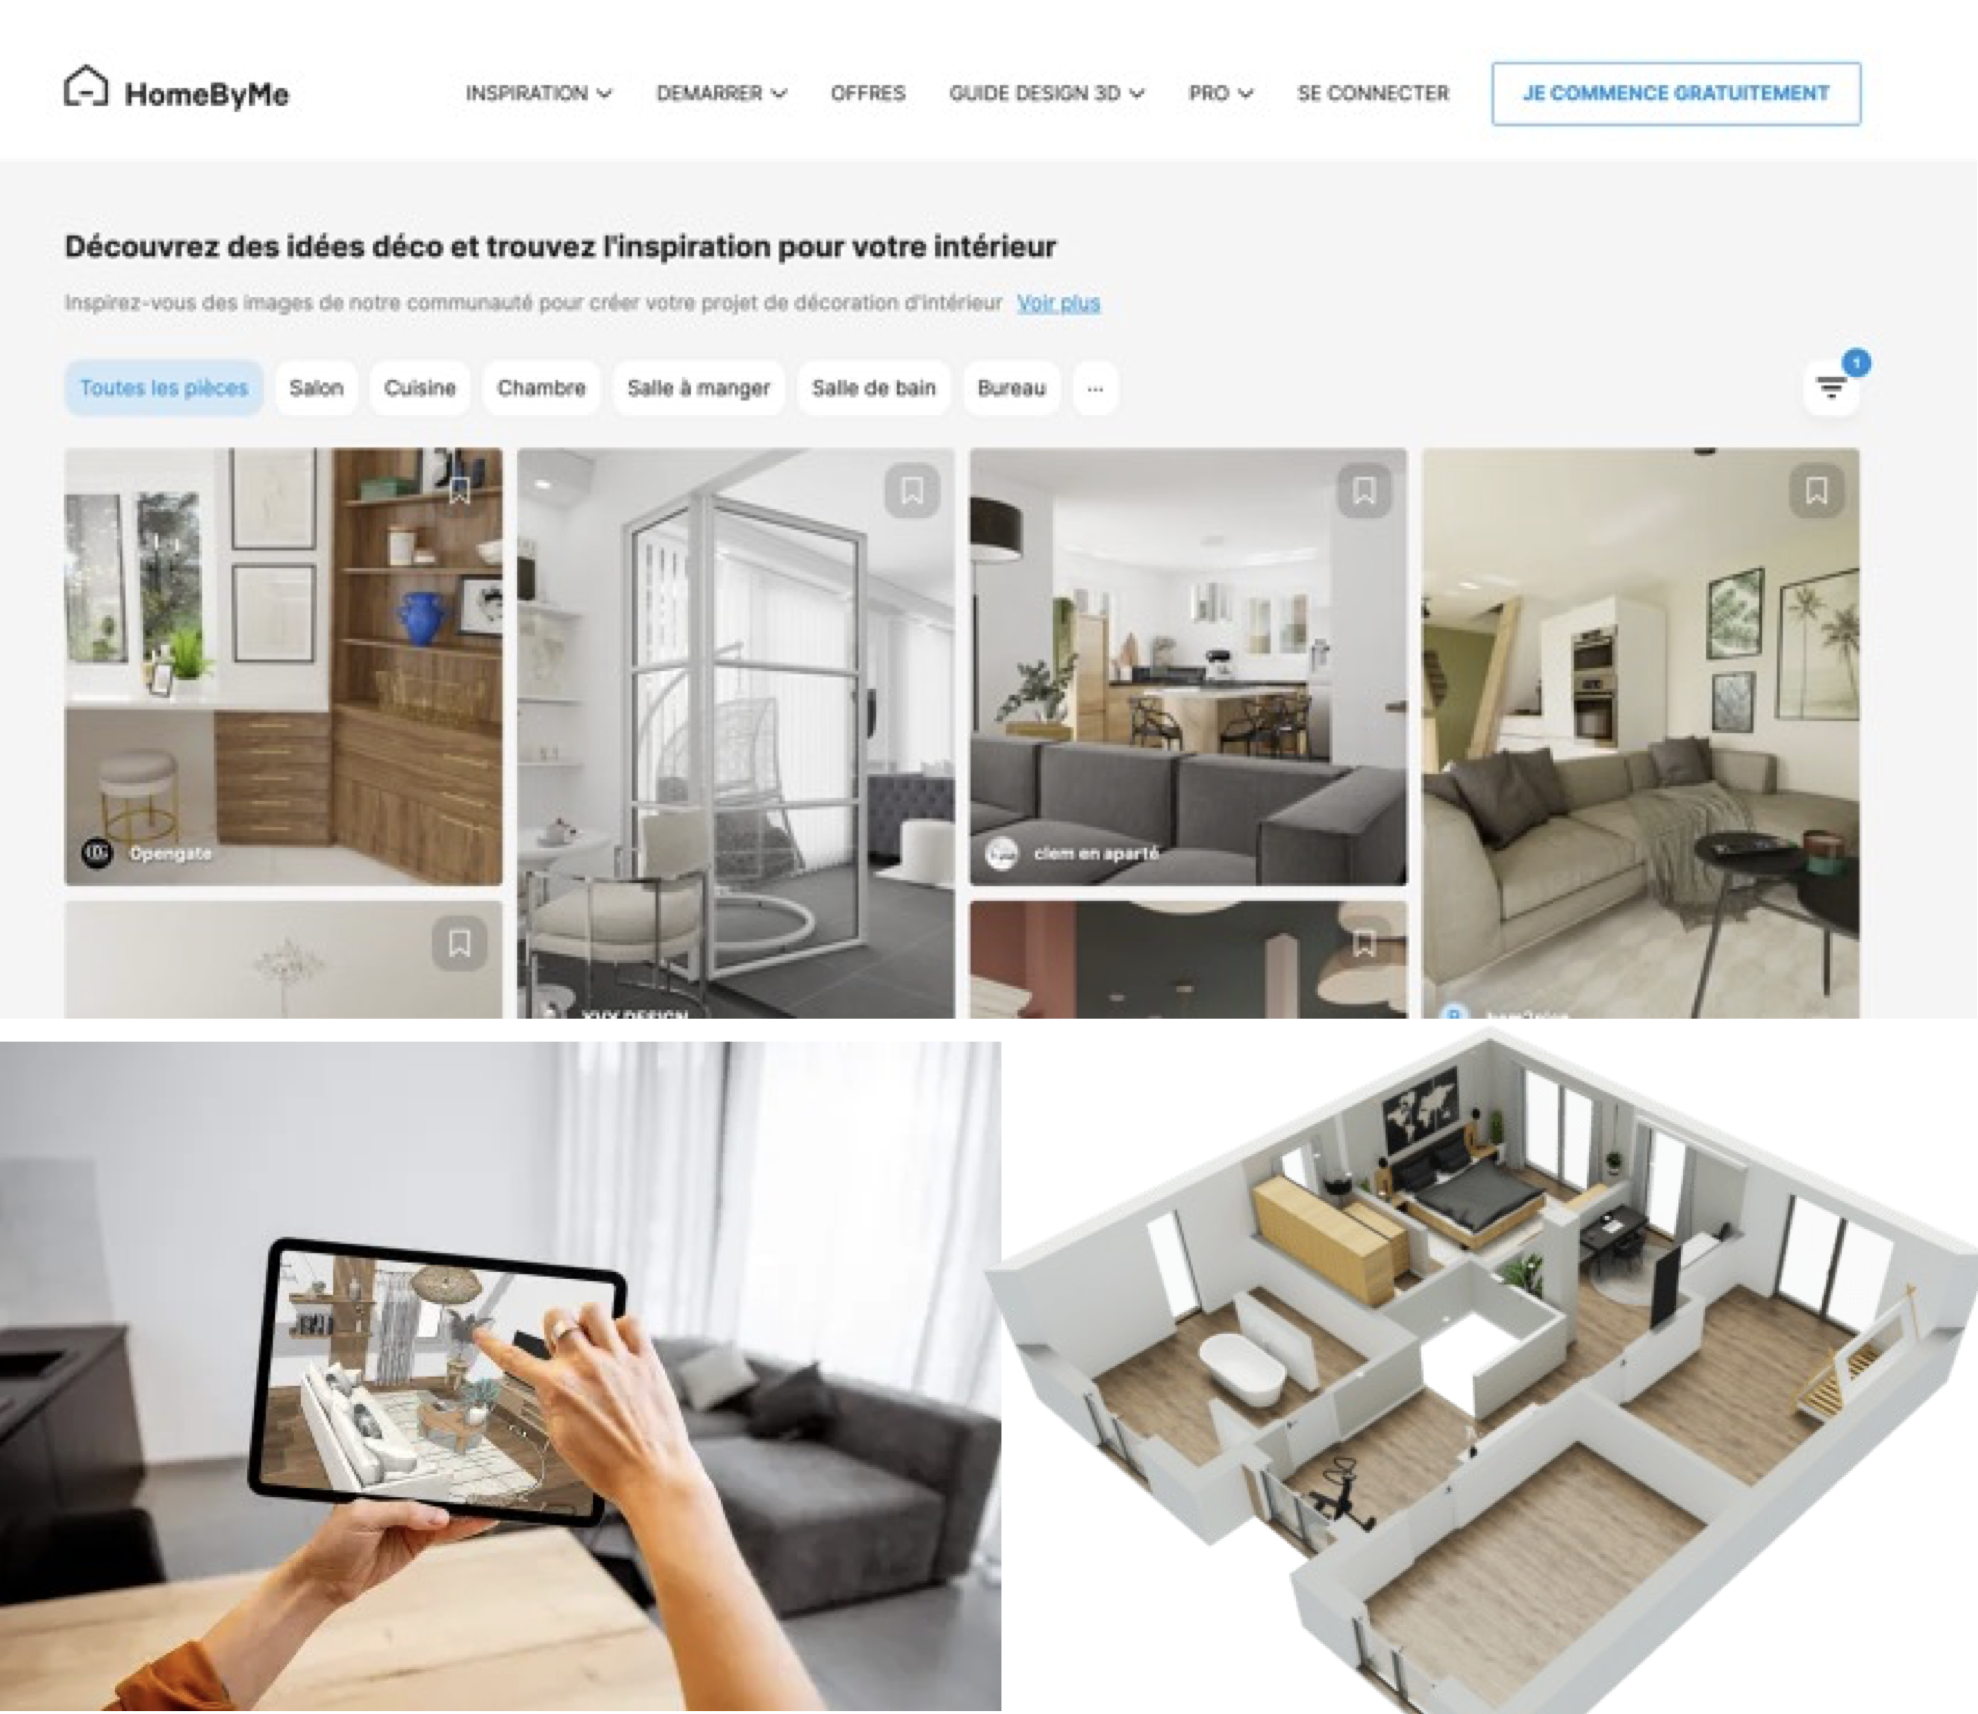
\includegraphics[width=\textwidth, height=15cm]{templateLatex/logos/HomeByMe.png}
      \end{figure}
      \begin{figure}
        \includegraphics[width=\textwidth, height=10cm]{templateLatex/logos/Jumeau virtuel.png}
      \end{figure}
        
      % \begin{alertblock}{Le Mans}
      %   Le Mans est le chef-lieu du département de la Sarthe: on y faisait grand commerce de volailles engraissées. On disait des manceaux bien portants qu'ils valaient $1.5$ normand.
      % \end{alertblock}
    \end{column}

    \begin{column}{\sepwidth}\end{column}
  \end{columns}

  % ------------ Horizontal separation for changing number of columns in the width ------------

  \begin{columns}[c] 
    \begin{column}{\sepwidth}\end{column} % Empty spacer column
  \end{columns}

  % ------------ Changing number of columns in the width ------------


  \begin{columns}[c] 
    \begin{column}{\sepwidth}\end{column} % Empty spacer column

    \begin{column}{\onecolwidth}
      \begin{block}{Problématique}
        % Cependant un Faucon sur sa perche voyait -- 
        % Notre Manceau qui s’enfuyait. -- 
        % Les chapons ont en nous fort peu de confiance, --  
        % Soit instinct, soit expérience.\newline
        % Celui-ci, qui ne fut qu’avec peine attrapé, -- 
        % Devait, le lendemain, être d’un grand souper, -- 
        % Fort à l’aise en un plat, honneur dont la volaille -- 
        % Se serait passée aisément.
        Les processus d'IA nécessitent une maintenance régulière à cause de changement récurrents des données sur lequel les modèles ont été entraînés pour garder une bonne performance, mais à l'échelle industrielle la gestion et la maintenance devient ingérable avec le grand volume des données et la nécessité du traitement en temps réel. Tout en assurant la sécurité et protection des données contre les cyberattaques ainsi que leur conformité, d'où le besoin de la mise en place d'un processus automatisé.

      \end{block}
    \end{column}

    \begin{column}{\sepwidth}\end{column} % Empty spacer column
  \end{columns}

  % ------------ Changing number of columns in the width ------------


  \begin{columns}[c]
    \begin{column}{\sepwidth}\end{column} % Empty spacer column

    \begin{column}{\fourcolwidth}
      \begin{block}{Machine Learning Operations (MLOps)}
      Le MLOps représente des méthodes et pratiques pour la gestion des projets d’IA, le but est l'automatisation et simplification du cycle de vie de l’IA.\\ Il s'agit de l'application des pratiques du DevOps sur le Machine Learning (ML)
      \end{block}

      \begin{block}{Mission}
        Ma mission principale en tant que stagiaire R\&D est de concevoir et mettre en place un processus robuste et automatisé pour maintenir les modèles à jour(utilisés pour la fontionalité de furniture detection), assurer une traçabilité complète des modèles et des données, automatiser le processus de machine learning à l’échelle industrielle, et la mise en place de systèmes de surveillance pour observer les métriques des modèles en production. 

      \end{block}

    \end{column}

    \begin{column}{\sepwidth}\end{column} % Empty spacer column

    \begin{column}{\twocolwidth}
      \vfill
      \begin{figure}
        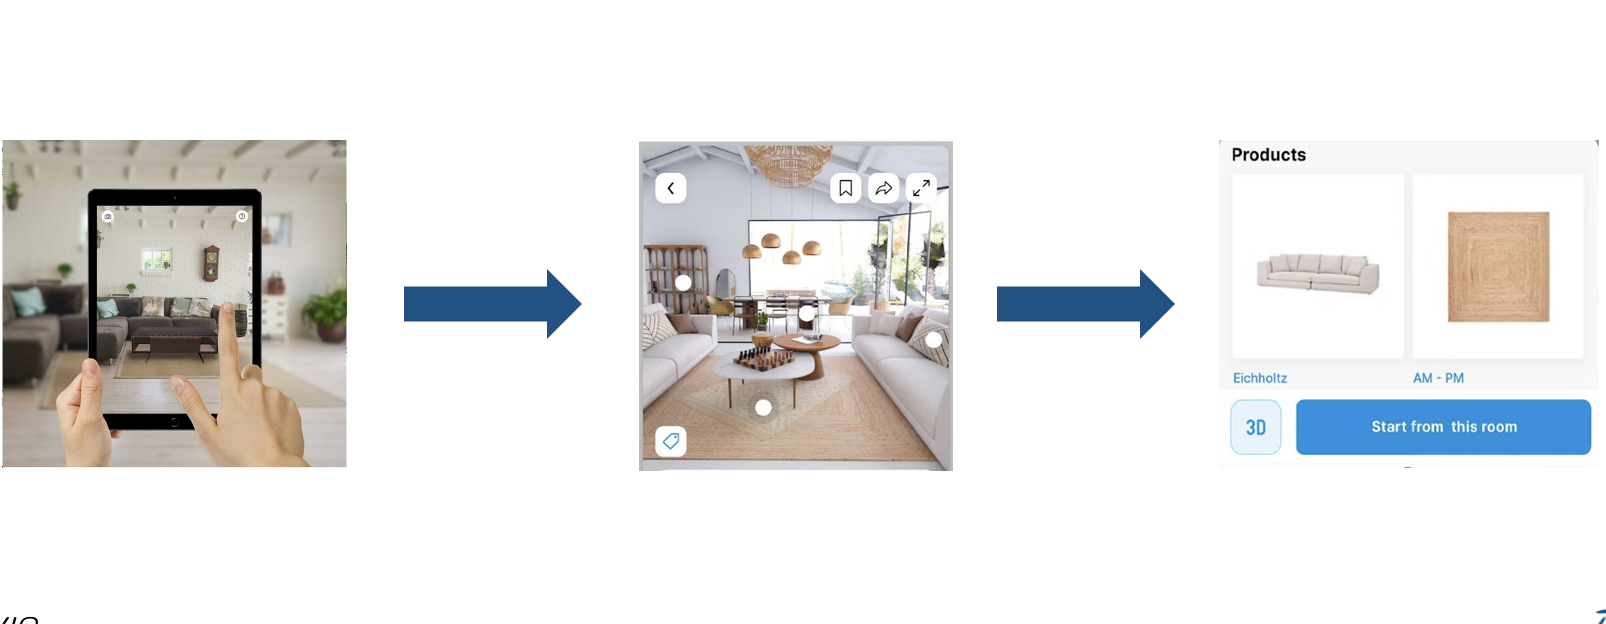
\includegraphics[width=\textwidth]{templateLatex/logos/furniture detection.png}
      \end{figure}

      \vfill
      \begin{block}{Fonctionnalité de detection de fourniture}
        Cette fonctionnalité
      \end{block}
      \vfill
    \end{column}

    \begin{column}{\sepwidth}\end{column} % Empty spacer column

    \begin{column}{\fourcolwidth}
      \begin{block}{La conclusion du Chapon}

        \begin{quote}
          Si tu voyais mettre à la broche \newline
          Tous les jours autant de faucons \newline
          Que j’y vois mettre de chapons, \newline
          Tu ne me ferais pas un semblable reproche. 
        \end{quote}
      \end{block}

      \begin{exampleblock}{Oiseau Tikz}
        \begin{figure}[ht!]
          \begin{center}
            \begin{tikzpicture}[scale=1.2,style=thick]
  \def\vr{2pt} % \vr = vertex radius;  Set \vr = 2/scale for uniform sizing
  of vertices
  %%% define points
  \path (0,0) coordinate (x);
  %%%


  \path (x) +(-180-180/11:3) coordinate (v1);
  \path (x) +(-180-180*2/11:3) coordinate (v2);
  \path (x) +(-180-180*3/11:3) coordinate (v3);
  \path (x) +(-180-180*4/11:3) coordinate (v4);
  \path (x) +(-180-180*5/11:3) coordinate (v5);
  \path (x) +(-180-180*6/11:3) coordinate (v6);
  \path (x) +(-180-180*7/11:3) coordinate (v7);
  \path (x) +(-180-180*8/11:3) coordinate (v8);
  \path (x) +(-180-180*9/11:3) coordinate (v9);
  \path (x) +(-180-180*10/11:3) coordinate (v10);
  %%%
  \path (x) +(-180-180*1.5/11:3.5) coordinate (w1);
  \path (x) +(-180-180*2.5/11:3.5) coordinate (w2);
  \path (x) +(-180-180*3.5/11:3.5) coordinate (w3);
  \path (x) +(-180-180*4.5/11:3.5) coordinate (w4);
  \path (x) +(-180-180*5.5/11:3.5) coordinate (w5);
  \path (x) +(-180-180*6.5/11:3.5) coordinate (w6);
  \path (x) +(-180-180*7.5/11:3.5) coordinate (w7);
  \path (x) +(-180-180*8.5/11:3.5) coordinate (w8);
  \path (x) +(-180-180*9.5/11:3.5) coordinate (w9);
  %%%
  \path (x) +(-180-180*1.8/11:4) coordinate (a2);
  \path (x) +(-180-180*2.2/11:4) coordinate (b2);
  \path (x) +(-180-180*2.8/11:4) coordinate (a3);
  \path (x) +(-180-180*3.2/11:4) coordinate (b3);
  \path (x) +(-180-180*3.8/11:4) coordinate (a4);
  \path (x) +(-180-180*4.2/11:4) coordinate (b4);
  \path (x) +(-180-180*4.8/11:4) coordinate (a5);
  \path (x) +(-180-180*5.2/11:4) coordinate (b5);
  \path (x) +(-180-180*5.8/11:4) coordinate (a6);
  \path (x) +(-180-180*6.2/11:4) coordinate (b6);
  \path (x) +(-180-180*6.8/11:4) coordinate (a7);
  \path (x) +(-180-180*7.2/11:4) coordinate (b7);
  \path (x) +(-180-180*7.8/11:4) coordinate (a8);
  \path (x) +(-180-180*8.2/11:4) coordinate (b8);
  \path (x) +(-180-180*8.8/11:4) coordinate (a9);
  \path (x) +(-180-180*9.2/11:4) coordinate (b9);
  \path (x) +(-180-180*9.8/11:4) coordinate (a10);
  \path (x) +(-180-180*10.2/11:4) coordinate (b10);
  \path (x) +(-180-180*10.6/11:4) coordinate (c10);
  %%% body of the peacock
  \path (-0.5,-0.6) coordinate (leg1);
  \path (-0.2,-1) coordinate (leg2);
  \path (0.2,-1) coordinate (leg3);
  \path (0.5,-0.6) coordinate (leg4);
  %%% Edges:
  \draw (v1) -- (x) -- (v2);
  \draw (v3) -- (x) -- (v4);
  \draw (v5) -- (x) -- (v6);
  \draw (v7) -- (x) -- (v8);
  \draw (v9) -- (x) -- (v10);
  %%%
  \draw (v1) -- (w1) -- (v2) -- (w2) -- (v3) -- (w3) -- (v4) -- (w4) -- (v5) -- (w5) -- (v6) -- (w6) -- (v7) -- (w7) -- (v8) -- (w8) -- (v9) -- (w9) -- (v10);
  %%%
  \draw (a2) -- (v2) -- (b2);
  \draw (a3) -- (v3) -- (b3);
  \draw (a4) -- (v4) -- (b4);
  \draw (a5) -- (v5) -- (b5);
  \draw (a6) -- (v6) -- (b6);
  \draw (a7) -- (v7) -- (b7);
  \draw (a8) -- (v8) -- (b8);
  \draw (a9) -- (v9) -- (b9);
  \draw (a10) -- (v10) -- (b10);
  \draw (v10) -- (c10);
  %%%
  \draw (leg1) -- (leg2) -- (leg3) -- (leg4);
  \draw (leg1) -- (x) -- (leg2);
  \draw (leg3) -- (x) -- (leg4);
  %%% Vertices:
  \draw (x) [fill=white] circle (\vr);
  \draw (v1) [fill=white] circle (\vr); \draw (v2) [fill=white] circle (\vr);
  \draw (v3) [fill=white] circle (\vr); \draw (v4) [fill=white] circle (\vr);
  \draw (v5) [fill=white] circle (\vr); \draw (v6) [fill=white] circle (\vr);
  \draw (v7) [fill=white] circle (\vr); \draw (v8) [fill=white] circle (\vr);
  \draw (v9) [fill=white] circle (\vr); \draw (v10) [fill=white] circle (\vr);
  %%%
  \draw (w1) [fill=white] circle (\vr); \draw (w2) [fill=white] circle (\vr);
  \draw (w2) [fill=white] circle (\vr); \draw (w3) [fill=white] circle (\vr);
  \draw (w4) [fill=white] circle (\vr); \draw (w5) [fill=white] circle (\vr);
  \draw (w6) [fill=white] circle (\vr); \draw (w7) [fill=white] circle (\vr);
  \draw (w8) [fill=white] circle (\vr); \draw (w9) [fill=white] circle (\vr);
  %%%
  \draw (a2) [fill=white] circle (\vr); \draw (b2) [fill=white] circle (\vr);
  \draw (a3) [fill=white] circle (\vr); \draw (b3) [fill=white] circle (\vr);
  \draw (a4) [fill=white] circle (\vr); \draw (b4) [fill=white] circle (\vr);
  \draw (a5) [fill=white] circle (\vr); \draw (b5) [fill=white] circle (\vr);
  \draw (a6) [fill=white] circle (\vr); \draw (b6) [fill=white] circle (\vr);
  \draw (a7) [fill=white] circle (\vr); \draw (b7) [fill=white] circle (\vr);
  \draw (a8) [fill=white] circle (\vr); \draw (b8) [fill=white] circle (\vr);
  \draw (a9) [fill=white] circle (\vr); \draw (b9) [fill=white] circle (\vr);
  \draw (a10) [fill=white] circle (\vr); \draw (b10) [fill=white] circle (\vr);
  \draw (c10) [fill=white] circle (\vr);
  %%% 
  \draw (leg1) [fill=white] circle (\vr);
  \draw (leg2) [fill=white] circle (\vr);
  \draw (leg3) [fill=white] circle (\vr);
  \draw (leg4) [fill=white] circle (\vr);
  %%% text
  \draw (-0.4,-0.1) node {$x$};
  \draw [below] (v1) node {$v_1$};
  \draw [below] (v2) node {$v_2$};
  \draw [below] (v9) node {$v_9$};
  \draw [below] (v10) node {$v_{10}$};
  \draw [left] (w1) node {$w_1$};
  \draw (w2) node[xshift=-8pt, yshift=12pt] {$w_2$};
  \draw (w9) node[xshift=8pt, yshift=2pt] {$w_9$};
  \draw [left] (leg1) node {$u_1$};
  \draw (-0.5,-1.2) node {$u_2$};
  \draw (0.5,-1.2) node {$u_3$};
  \draw [right] (leg4) node {$u_4$};
\end{tikzpicture}

          \end{center}
        \end{figure}
        Certes cet oiseau ne ressemble ni à un chapon, ni à un faucon. Léon! Serait-ce un Paon?
      \end{exampleblock}

    \end{column}

    \begin{column}{\sepwidth}\end{column} % Empty spacer column
  \end{columns}

\end{frame}

\end{document}
